\documentclass[a4paper,11pt]{article}
\usepackage{jinstpub} % for details on the use of the package, please see the JINST-author-manual
\usepackage{lineno}
\usepackage{bm}
\usepackage{mathtools}
\usepackage{comment}
\linenumbers

% Custom commands
\newcommand{\strutlike}{\rule{0pt}{1.1\normalbaselineskip}}

\title{\boldmath Goodness-of-fit for multi-distribution neutrino cross-section measurements with shared events}

\author{F. Mart\'inez L\'opez}
\affiliation{Department of Physics, Indiana University,\\727 E. Third St., Bloomington, IN, USA, 47405}

% E-mail addresses: only for the corresponding author
\emailAdd{frmar@iu.edu}

\abstract{When multiple differential cross-section distributions are extracted from a common event sample with correctly evaluated inter-distribution correlations, the statistical covariance matrix is generically singular. Exact linear constraints from event sharing across measurements, such as equal distribution totals when all selected events populate bins in every distribution, produce directions with zero statistical variance. Systematic uncertainties restore formal invertibility but leave near-singular directions that yield unphysically inflated $\chi^{2}$ values in global goodness-of-fit tests. We present a projection method that restricts the test to the subspace carrying independent statistical information, yielding a $\chi^{2}$ distributed with $N_\text{bins} - N_\text{null}$ degrees of freedom, where $N_\text{null}$ is the number of independent constraints. The method is connected to established results on hypothesis testing with singular covariance matrices and validated with both an analytical toy model and a realistic simulated neutrino--argon cross-section measurement including unfolding and parametrized multi-source systematic uncertainties.}

\keywords{Analysis and statistical methods}

\arxivnumber{1234.56789} % Only if you have one

\begin{document}
\maketitle
\flushbottom

\section{Introduction}

% Opening paragraph -- multi-distribution xsec measurements
Modern neutrino cross-section literature is experiencing an increase of published measurements reporting multiple differential distributions extracted from the same event sample. MicroBooNE has reported simultaneous measurements of cross sections for final states with and without protons \cite{MicroBooNE:2024zkh,MicroBooNE:2024zwf}, multi-differential QE-like cross section measurements in kinematic imbalance variables \cite{MicroBooNE:2023tzj,MicroBooNE:2023cmw}, and triple-differential inclusive results \cite{MicroBooNE:2023foc}. Other relevant examples include the multiple final-state kinematic projections from T2K \cite{T2K:2018rnz,T2K:2021naz}, and double-differential inclusive results from NOvA \cite{NOvA:2021eqi,NOvA:2024zmr,NOvA:2024rov}. In each of these analyses, the same selected events populate bins in multiple reported distributions, leading to strong inter-measurement statistical correlations. Separate but related efforts have produced simultaneous measurements across different nuclear targets \cite{T2K:2020jav,MINERvA:2023kuz,MINERvA:2022djk} and combined neutrino-antineutrino results \cite{T2K:2020sbd}, where correlations arise from shared systematic uncertainties rather than shared events.

% Blockwise unfolding intro
The blockwise unfolding framework \cite{Gardiner:2024gdy} provides a rigorous method for computing the full cross-distribution covariance matrices in all such measurements. In this approach, all bins corresponding to the same measured observable in the multi-distribution analysis are organized in blocks, each corresponding to a single differential cross-section distribution. Each bin block is unfolded independently using any standard method (e.g. iterative D'Agostini unfolding \cite{DAgostini:1994fjx} or Wiener-SVD \cite{Tang:2017rob}), while the full covariance matrix, encoding the correlations between bins from different distributions, is constructed and propagated through the cross section extraction procedure. The statistical covariance for bins in different blocks is determined by the number of events they share. The result is a single combined covariance matrix covering all reported bins across all distributions.

% Global goodness-of-fit
A natural use of these combined measurements is computing global goodness-of-fit metrics, such as a $\chi^{2}$ statistic, that test a model against all distributions simultaneously. Compared to evaluating each distribution independently, a global test that accounts for all inter-block correlations provides the maximum discriminating power available from the data. Such global metrics are essential for interaction model tuning efforts \cite{Wilkinson:2016wmz,MINERvA:2019kfr,GENIE:2022qrc}, where measurements of multiple kinematic distributions provide complementary sensitivity to different aspects of the underlying physics. However, as we show in this paper, the full inter-block statistical covariance is generically singular when it correctly accounts for correlations from shared events. The rank deficiency arises from exact linear constraints imposed by the event-sharing structure of the binning scheme: certain linear combinations of bins, such as the difference in total event counts between two distributions of the same events, have identically zero variance. While systematic uncertainties formally restore invertibility, the resulting near-singular directions produce unphysically inflated $\chi^{2}$ values, yielding a global test with the wrong effective number of degrees of freedom.

% Motivation for paper
We present a method based on projecting onto the range (column space) of the statistical covariance matrix that yields a well-defined chi-squared with the correct number of degrees of freedom. We demonstrate the method using a pedagogical toy example and connect it to the established statistical literature on hypothesis testing with singular covariance matrices.

% Outline
Brief roadmap of sections.

\section{Rank deficiency of the statistical covariance}

Consider a neutrino cross-section analysis simultaneously measuring $B$ different flux-integrated differential cross sections, each with $N_b$ true bins. If the measurement is extracted from a common event sample then each selected event will populate exactly one bin in each distribution it belongs to. Recent MicroBooNE analyses \cite{MicroBooNE:2024yzp} have adopted the blockwise unfolding approach presented in Ref. \cite{Gardiner:2024gdy} to simultaneous cross-section measurements.

This method provides a systematic framework for reporting the correlations between the different extracted differential cross sections. It provides a general prescription to construct statistical covariance matrices that respect the correlations between bins in different distributions or blocks. The full inter-block covariance matrix constructed in reconstructed space is propagated through unfolding using a block-diagonal unfolding matrix, obtained as a direct sum of the individual unfolding matrices computed for each block. The result of the combined measurement is a vector of $N_{\text{bins}} = \sum_{b=1}^{B} N_b$ cross-section values with an $N_{\text{bins}} \times N_{\text{bins}}$ covariance matrix.

\subsection{Statistical covariance from shared events}

The core idea behind the treatment of the statistical correlations in the blockwise unfolding approach is the partition of any arbitrary pair of overlapping kinematic bins $X$ and $Y$ into a set of three non-overlaping bins $u$, $v$, and $w$. The events in the intersection $X \cap Y$ are assigned to bin $v$, while bin $u$ contains the events in the relative complement of $Y$ in $X$ (i.e. $X \setminus Y$), and bin $w$ corresponds to the relative complement of $X$ in $Y$ (i.e. $Y \setminus X$). Denoting the number of predicted events in each bin as $n_{i}$, and assuming these follow independent Poisson distributions, the covariance between the counts in bins $X$ and $Y$ is given by \cite{Gardiner:2024gdy}:
\begin{equation}
    \begin{split}
        \text{Cov}(n_{X}, n_{Y}) &= \text{Cov}(n_{u} + n_{v}, n_{v} + n_{w})\\
        &= \text{Cov}(n_{u}, n_{v}) + \text{Cov}(n_{u}, n_{w}) + \text{Cov}(n_{v}, n_{v}) + \text{Cov}(n_{v}, n_{w})\\
        &= \text{Var}(n_{v}),
    \end{split}
\end{equation}
as by definition bins $u$, $v$, and $w$ have no events in common. This implies that the covariance between any two bins can be estimated from the variance of the events they share.

The variance for a set of Monte Carlo (MC) events can be estimated from the sum of their squared weights. This gives us a general prescription to calculate the elements of the statistical covariance matrix as:
\begin{equation}\label{eq:cstat_elements}
    (C_{\text{stat}})_{ij} = \sum_{e \in (i \cap j)} w_{e}^{2},
\end{equation}
where $w_{e}$ is the weight associated to event $e$ belonging to the intersection of bins $i$ and $j$. In the case of measured data the weights are $1$, and the covariance element simplifies to the number of events shared between the bins $n_{ij}$.

After propagation through the block-diagonal unfolding, the statistical covariance matrix in unfolded space inherits the same rank structure, as the unfolding matrices for each individual block are invertible. This rank structure has a direct interpretation in terms of the number of distinct event-sharing patterns across distributions, which we discuss next.

\subsection{Combination matrix and null space}

The previous discussion shows that the statistical covariance between any two bins is determined solely by the events they share. We now formalize this observation to derive an exact formula for the rank of $C_{\text{stat}}$, and therefore for the number of directions in bin space that carry zero statistical variance.

For each event $e$, we can define the indicator vector $\bm{\phi}_{e} \coloneqq (\phi_{e,i})_{i = 1}^{N_{\text{bins}}}$ such that $\phi_{e,i} = 1$ if $i \in \text{bins}(e)$ and $\phi_{e,i} = 0$ if $i \notin \text{bins}(e)$, where $\text{bins}(e)$ is the set of bins event $e$ populates across all distributions. The indicator vector acts as an identifier of each event in the combined measurement. For example, in a two-block measurement with 3 bins each, an event populating bin 2 of block 1 and bin 1 of block 2 has indicator vector $\bm{\phi}_{e} = (0,1,0,1,0,0)$. The statistical covariance matrix can then be re-written in terms of indicator vectors as:
\begin{equation}\label{eq:cstat_outer}
    C_{\text{stat}} = \sum_{e} w_{e}^{2} \, \bm{\phi}_{e} \, \bm{\phi}_{e}^{\mathsf{T}}.
\end{equation}

This outer-product decomposition makes the rank structure of $C_{\text{stat}}$ clear. The rank of the statistical covariance matrix equals the dimension of $\mathrm{span}\{\bm{\phi}_e\}$, which depends only on the distinct indicator vectors present, not on their weights. Since all weights are $w_{e} > 0$ no indicator vector is removed from the sum, and the column space of $C_{\text{stat}}$ is exactly $\mathrm{span}\{\bm{\phi}_e\}$.

We define the bin-combination matrix $A$ as the matrix whose rows are the unique indicator vectors among $\{\bm{\phi}_e\}$. Each row of $A$ represent a distinct pattern of bin occupancy across the blocks. By construction the row space of $A$ equals $\mathrm{span}\{\bm{\phi}_e\}$, and therefore:
\begin{equation}\label{eq:rank_formula}
    \mathrm{rank} (C_{\text{stat}}) = \mathrm{rank} (A).
\end{equation}
The number of degenerate directions is then:
\begin{equation}\label{eq:nnull}
    N_{\text{null}} = N_{\text{bins}} - \mathrm{rank} (A).
\end{equation}

Physically, each of the $N_{\text{null}}$ directions corresponds to a linear combination of bins along which the measurement has identically zero variance. Any component of the residual vector along such a direction is not perceived by the statistical covariance; it is a direction that the measurement has no statistical power to constrain. Importantly, both $A$ and $N_{\text{null}}$ are directly computable from the MC event-to-bin mapping alone, before constructing any covariance matrix.

A vector $\mathbf{x}$ is in the null space of $C_{\text{stat}}$ if and only if, for every event $e$:
\begin{equation}\label{eq:null_condition}
    \sum_{i \in \text{bins}(e)} x_{i} = 0,
\end{equation}
or equivalently $A \mathbf{x} = 0$. Each unique indicator vector acts as a linear constraint on the null-space vectors, requiring that the components of $\mathbf{x}$ sum to zero over the bins populated by the different events. The null space directions can be divided into two physically distinct categories: structural constraints that follow from the block topology alone, and kinematic constraints that depend on which regions of phase space are populated.

\subsection{Determination of the structural null space}

The combination matrix $A$ presented previously is constructed from MC events. One determines which events populate the different bins and collects the unique indicator vectors. However, the indicator vectors that can appear are constrained by two distinct mechanisms. The first is purely structural, the geometry of the binning scheme forbids certain bin combinations. The second is kinematic, correlations between the different variables render some combinations unreachable even though they are geometrically allowed. These constraints are imposed by the underlying physics effects, mainly the differential cross section and the detector acceptance. In the following, we show that the structural constraints can be determined a priori, without generating MC events, from the bin edges used.

The variables used in a measurement are drawn from a set $\{v_{1}, \ldots v_{D}\}$. Each block $b$ uses a subset of these variables, $\mathrm{vars}(b) \subseteq \{v_{1}, \ldots v_{D}\}$. Restricting the discussion to combinations of single- and double-differential measurements, we have $|\mathrm{vars}(b)| \in \{1,2\}$ for every $b$. For each variable $v$ used in a given block $b$, the binning scheme defines a set of bin edges $E_{v}^{(b)}$ that partition the range of $v$ into intervals. In the case of a two-dimensional block, the edges in the binning variable may be slice-dependent, but nevertheless these can be collected into a single set of edges per variable across slices. For each variable $v \in \bigcup_{b} \mathrm{vars}(b)$, we can define the refined edges:
\begin{equation}
    \mathcal{E}_{v} = \bigcup_{b \, : \, v \in \mathrm{vars}(b)} E_{v}^{(b)},
\end{equation}
with $M_{v} = |\mathcal{E}_{v}| - 1$ denoting the number of refined bins for variable $v$. Since $\mathcal{E}_{v}$ contains all the bin edges from every block that uses that variable, each refined bin is contained entirely within one original bin of every such block.

The common refinement of all blocks is the Cartesian product of the refined bins across all variables:
\begin{equation}
    \mathcal{R} = \bigtimes_{v} \{1,\ldots,M_v\}.
\end{equation}
Each cell $c \in \mathcal{R}$ specifies a refined bin index for every variable in the measurement. For every block $b$, there exists a unique mapping $\beta_{b}(c)$ between each cell $c$ and an original bin in said block. The elements of the indicator vector $\bm{\phi}_{c} \coloneqq (\phi_{c,i})_{i=1}^{N_{\text{bins}}}$ associated to cell $c$ can be written as:
\begin{equation}
    \phi_{c,i} = \begin{cases}
        1 & \text{if } i = \beta_b(c) \text{ for any block } b, \\
        0 & \text{otherwise.}
    \end{cases}
\end{equation}
If block $b$ does not use variable $v$ then $\beta_{b}$ is independent of the refined bin index in $v$. Therefore, multiple cells may produce identical indicator vectors.

The structural combination matrix $A_{\text{struct}}$ is defined as the matrix whose rows are the unique indicator vectors from the cells of the common refinement $\{\bm{\phi}_{c} \, : \, c \in \mathcal{R}\}$. By construction, every indicator vector that appears in the $A$ matrix obtained from the MC events is also present in $A_{\text{struct}}$, therefore:
\begin{equation}
    \mathrm{rank}(A) \leq \mathrm{rank}(A_{\text{struct}}) \leq N_{\text{bins}}.
\end{equation}
This hierarchy motivates a decomposition of the total number of degenerate directions:
\begin{equation}
    \begin{split}
        N_{\text{null}} &= N_{\text{bins}} - \mathrm{rank}(A_{\text{struct}}) + \mathrm{rank}(A_{\text{struct}}) - \mathrm{rank}(A)\\
        &= N_{\text{null}}^{\text{struct}} + N_{\text{null}}^{\text{kinem}}.
    \end{split}    
\end{equation}
The first term, $N_{\text{null}}^{\text{struct}}$, counts null directions that arise purely from the binning geometry and is computable a priori from the bin edges alone. The second term, $N_{\text{null}}^{\text{kinem}}$, accounts for additional null directions introduced by phase-space restrictions that exclude geometrically allowed combinations and can only be determined from Monte Carlo. A description of the algorithm used to compute $A_{\text{struct}}$, including an optimization that restricts the enumeration to shared variables, is presented in Appendix \ref{app:algorithm}.

The structure of the null space of $A_{\text{struct}}$ depends on how the bin edges for the different blocks overlap. In the simplest case, when blocks do not share variables, every combination of one bin per block is allowed. The resulting null space is $(B-1)$-dimensional, with a single constraint that requires all block totals to be equal. When blocks share one or more variables, the allowed combinations are restricted and the dimension of the null space can be different from $B-1$. The number of null directions depends on how shared variable bin edges are aligned between blocks. Aligned slice edges decouple the measurement into different sub-problems, adding additional sum rules and increasing $N_{\text{null}}^{\text{struct}}$. On the other hand, misaligned edges couple adjacent distributions, potentially reducing the number of constraints. In the general case, the interplay between shared variables, bin edge alignment, and block topology makes a closed-form expression impractical, but the computation of $\mathrm{rank}(A_{\text{struct}})$ from the bin edge specifications is straightforward.

The structural and kinematic components of the null space respond differently to systematic uncertainties. Whether these cause the rank deficiency of $C_{\text{stat}}$ to persist, partially resolve, or fully resolve in the total covariance $C_{\text{total}}$ depends on the nature of the systematic treatment, which we discuss next.

\begin{comment}
The number of null directions $N_\text{null}$ depends on the overlap structure between blocks. The constraints described above hold exactly when every selected event populates at least one bin in every block, as is the case when underflow and overflow bins are included. Without such bins, events falling outside the kinematic range of a given block do not contribute to the inter-block sum rules, potentially reducing $N_\text{null}$. In practice, the inclusion of overflow bins is already recommended for proper unfolding closure \cite{Gardiner:2024gdy}, and any well-designed blockwise analysis will therefore exhibit the full set of constraints. The projection method presented here remains valid regardless of the value of $N_\text{null}$, including the limiting case $N_\text{null} = 0$ where $C_\text{stat}$ is full rank and the projector reduces to the identity.
\end{comment}

\subsection{Effect of systematic uncertainties}

\subsection{Ignoring inter-block correlations}

\section{Range projection method}

the SVD decomposition of the statistical covariance matrix as:
\begin{equation}
    C_{\text{stat}} = U \, \Sigma \, U^{\mathsf{T}},
\end{equation}
and that $r = \mathrm{rank}(C_{\text{stat}})$. partitionings of $U = [U_{r} | \bar{U}_{r}]$
\begin{equation}
    \begin{split}
        U_{r} U_{r}^{T} &= \text{projection on to } \mathrm{ran}(C_{\text{stat}})\\
        \bar{U}_{r} \bar{U}_{r}^{T} &= \text{projection on to } \mathrm{null}(C_{\text{stat}})
    \end{split}
\end{equation}

\subsection{Constructing the projector}

\subsection{Projected chi-squared}

\subsection{Proof sketch / justification}

\subsection{Relation to alternative approaches}

\section{Analytical demonstration}

\begin{figure}[!h]
	\centering
	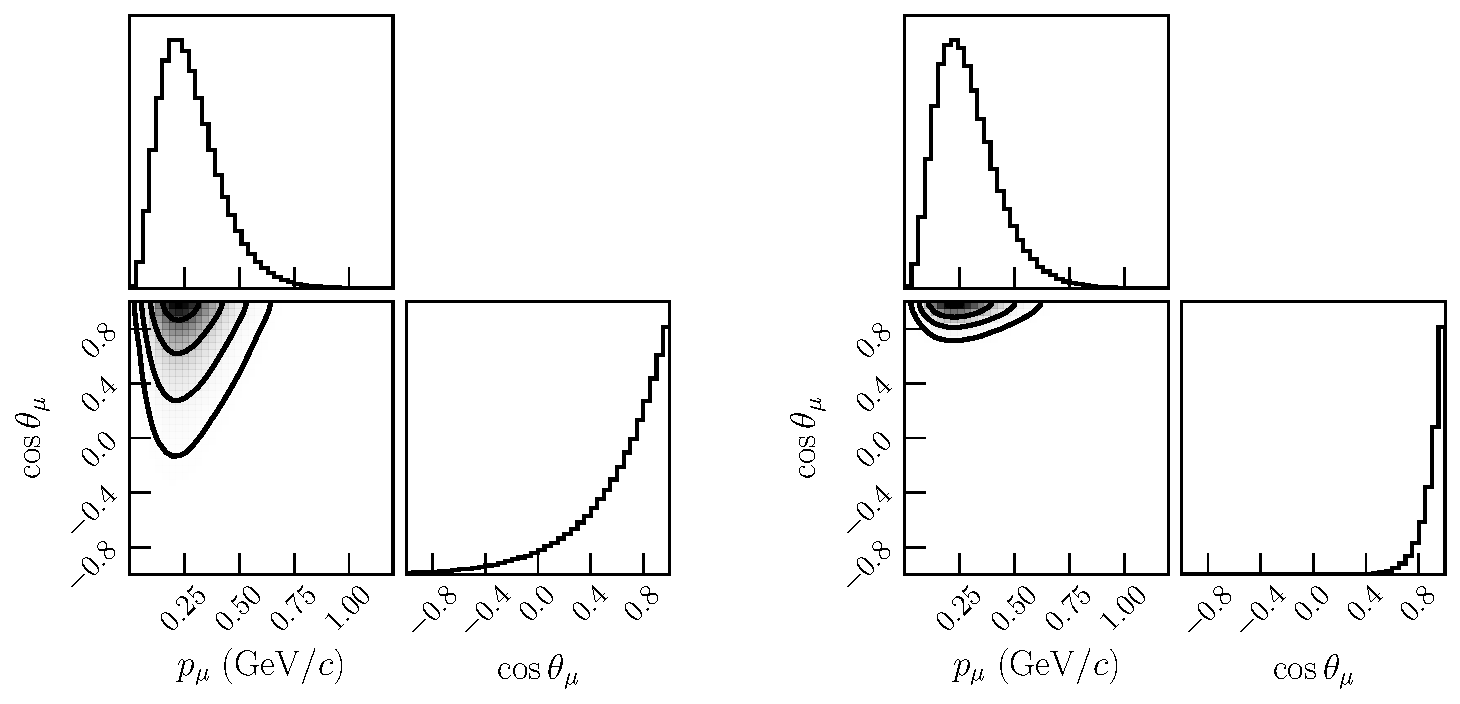
\includegraphics[width=1.00\linewidth]{images/analytical_corner_example.pdf}
	\caption{Expected number of signal events for reconstructed bins in block 11, used for the double-differential $(N_{p}, ~\mathrm{cos}~\theta_{\mu l_{4}})$ measurement. Both the central-value MicroBooNE tune prediction (black line) and the NuWro alternative prediction (blue line) are shown. Error bars include only the MC statistical uncertainty.}
	\label{fig:analytical_corner_example}
\end{figure}

\subsection{Setup}

\subsection{Eigenvalue analysis}

\subsection{Pseudo-experiment validation}

\subsection{Sensitivity to threshold choice}

\section{Realistic demonstration with neutrino generators }

\subsection{Simulation setup}

\subsection{Example 1: Two blocks ($N_{\text{null}} = 1$)}

\subsection{Example 2: Four blocks with multiplicity slicing ($N_{\text{null}} = 2$)}

\subsection{Practical observations}

\section{Practical implementation guide}

\subsection{Step-by-step recipe}

\subsection{What to include in data releases}

\subsection{Compatibility notes}

\section{Connection to the statistics literature}

\section{Summary and recommendations}

\acknowledgments

\appendix
\section{Algorithm}
\label{app:algorithm}

The naive counting of the common refinement $\mathcal{R}$ has cost $\prod_{v} M_{v}$, which grows exponentially with the number of kinematic variables. A typical multi-distribution measurement involves $\mathcal{O}(5)$ variables each with $\mathcal{O}(10)$ refined bins, giving $\mathcal{O}(10^{5})$ cells. The key insight is that only shared variables (i.e. the ones appearing in two or more blocks) generate the cross-block constraints. Dividing the variable set into shared ($V_{s}$) and private ($V_{p}$) variables, one has to enumerate only the reduced refinement $\prod_{v \in V_{s}} M_{v}$. For each of the shared-variable cells, the bins from blocks that depend on the shared variable are determined by lookup, while blocks whose binning variable is private contribute their bins independently via a local Cartesian product. If the number of shared variables is small the computational cost is dramatically reduced.

% Bibliography

%% [A] Recommended: using JHEP.bst file
\bibliographystyle{JHEP}
\bibliography{biblio.bib}

\end{document}
